\chapter{पौधों में अलैंगिक जनन और क्लोनन}\label{ch:b2:asexual-reproduction}

यूटा की एक घाटी में ऐस्पन के सैंतालीस हज़ार तनों का एक वन खड़ा है जो एक
ही पौधा है: हर तना उसी एक मूल-तंत्र से उगा है, हर कोशिका वही जीनोम ढोती
है, और वह व्यक्ति कोई चौदह हज़ार वर्ष पुराना है तथा छह हज़ार टन भारी।
किसी दुकान में एक ही क़िस्म की स्ट्रॉबेरी की टोकरी की हर स्ट्रॉबेरी
भूस्तारियों से गुणित एक ही पौधे का टुकड़ा है; और पृथ्वी का हर कैवेंडिश
केला किसी एक पौधे की कलम की कलम है। पौधे, अधिकांश प्राणियों के विपरीत,
बिना लैंगिकता के नए व्यक्ति बना सकते हैं --- किसी तने से, किसी जड़ से,
किसी पत्ती से, किसी फ़्लास्क की एक कोशिका से। यह अध्याय देखता है कि वे
यह कैसे करते हैं, उगाने वाले इसका क्या उपयोग करते हैं, और किसी वंशक्रम
को \omterm{def:b2:meiosis-heredity:meiosis}{अर्धसूत्री विभाजन} तथा निषेचन छोड़ने का क्या दाम पड़ता है: यानी यह
प्रश्न कि लैंगिकता है ही क्यों।

\section{कायिक गुणन}

\begin{definition}[क्लोन, जेनेट, रैमेट]\label{def:b2:asexual-reproduction:clone}
\index{क्लोन}\index{जेनेट}\index{रैमेट}\index{कायिक गुणन}
\emph{अलैंगिक जनन} एक ही जनक से केवल समसूत्री विभाजन द्वारा, बिना
\omterm{def:b2:meiosis-heredity:meiosis}{अर्धसूत्री विभाजन} या निषेचन के, नए व्यक्ति बनाता है: वह संतति
एक \emph{क्लोन} है, जो जनक से और आपस में आनुवंशिक रूप से समरूप है, सिवाय
उन कायिक \omterm{def:b2:genome-diversification:mutation}{उत्परिवर्तनों} के जो जमा होते जाते हैं। पौधों में
सामान्य रूप \emph{कायिक गुणन} है, जिसमें शरीर का कोई भाग --- तना, जड़,
पत्ती --- जड़ पकड़कर एक अलग पौधा बन जाता है।
\emph{जेनेट} आनुवंशिक व्यक्ति है, यानी वह सब जो एक ही युग्मनज से उगा;
और \emph{रैमेट} उसकी एक शरीरक्रियात्मक रूप से अलग इकाई है।
स्ट्रॉबेरी की किसी क्यारी में एक ही जेनेट के हज़ार रैमेट हो सकते हैं; और
वह ऐस्पन वन एक ही जेनेट है। कायिक गुणन इसलिए संभव है कि पादप कोशिकाएँ
विभाजित होने और कोई भी अंग बनाने की क्षमता बनाए रखती हैं
--- वे \emph{पूर्णशक्त} हैं --- और इसलिए भी कि पौधे ऐसे
विभज्योतकों से उगते हैं जिन्हें लगभग कहीं भी फिर से जगाया जा सकता है।
\end{definition}

\begin{proposition}[कायिक गुणन के अंग]\label{prop:b2:asexual-reproduction:organs}
\index{भूस्तारी}\index{प्रकंद}\index{कंद}\index{शल्ककंद}
पौधों ने वही तरकीब हर अंग से विकसित की है। तनों से:
\emph{भूस्तारी} या \emph{स्टोलन}, यानी ज़मीन के साथ-साथ चलने वाले क्षैतिज
प्ररोह जो अपनी पर्वसंधियों पर जड़ पकड़ते हैं (स्ट्रॉबेरी, रेंगती
बटरकप); \emph{प्रकंद}, यानी क्षैतिज भूमिगत तने जो शाखित होते और टूटते
हैं (दूब, आइरिस, अदरक, ब्रेकन); \emph{कंद}, यानी प्रकंद के फूले हुए
सिरे जो मंड सँजोते हैं और कलिकाएँ, यानी ``आँखें'', ढोते हैं
(आलू); \emph{घनकंद}, यानी फूले हुए ऊर्ध्वाधर तना-आधार (क्रोकस);
\emph{कंदिकाएँ}, यानी पत्तियों के कक्ष में या
पुष्पगुच्छ में बने छोटे शल्ककंद (लहसुन, कुछ प्याज़)। पत्तियों से:
\emph{शल्ककंद}, यानी माँसल भंडार-पत्तियों में लिपटी कलिकाएँ जो फटकर
पुत्री-शल्ककंद बनाती हैं (प्याज़, ट्यूलिप); और पत्ती के किनारे उगते
पौधक, जड़ों समेत पूरे, जो झड़ जाते हैं (\emph{Kalanchoe})। जड़ों से:
\emph{मूल-प्ररोह}, यानी क्षैतिज जड़ों से उठते प्ररोह (ऐस्पन, काँटेदार
बेर, रसभरी)। \emph{खंडन} से: विलो की कोई टहनी जो बहकर दूर जाती और जड़
पकड़ती है, या कोई लेम्ना पर्ण जो बँट जाता है। हर स्थिति में कोई
भंडार-अंग या कोई विभज्योतक थोड़ी दूर ले जाया जाता है, और पुत्री अपना
जीवन ऐसे भोजन-भंडार से आरंभ करती है जिसकी बराबरी कोई \omterm{def:b2:angiosperm-reproduction:seed}{बीज} नहीं कर सकता।
\end{proposition}

\begin{omfigure}
\begin{tikzpicture}[every node/.style={font=\scriptsize}]
  % runner
  \begin{scope}
    \draw[thick] (0,0) -- (3.6,0);
    \foreach \x in {0,1.8} { \draw[thick, omExo!70!black, fill=omExo!30] (\x,0) .. controls (\x-0.3,0.6) and (\x+0.3,0.6) .. (\x,0); \foreach \a in {60,90,120} \draw[thick, omExo!70!black] (\x,0) -- ++(\a:0.7); \draw[gray] (\x,0) -- ++(-100:0.4) (\x,0) -- ++(-70:0.4); }
    \draw[thick, omThm] (0.2,0.15) .. controls (0.9,0.55) and (1.2,0.55) .. (1.8,0.1);
    \draw[thick, omThm] (2.0,0.15) .. controls (2.7,0.55) and (3.0,0.55) .. (3.5,0.1);
    \draw[thick, omExo!70!black] (3.5,0.1) -- ++(80:0.4); \draw[gray] (3.5,0.1) -- ++(-80:0.3);
    \node[below, align=center] at (1.8,-0.55) {भूस्तारी (स्ट्रॉबेरी):\\कोई क्षैतिज प्ररोह अपनी पर्वसंधियों पर जड़ पकड़ता है};
  \end{scope}
  % rhizome and tuber
  \begin{scope}[xshift=5.2cm]
    \draw[gray, dashed] (-0.2,0) -- (3.8,0);
    \draw[very thick, omProp!80!black] (0,-0.5) -- (3.4,-0.5);
    \foreach \x in {0.6,2.0} \draw[thick, omExo!70!black] (\x,-0.5) -- (\x,0.7) (\x,0.3) -- ++(40:0.4) (\x,0.3) -- ++(140:0.4);
    \draw[thick, omProp!80!black, fill=omProp!40] (3.4,-0.5) ellipse (0.45 and 0.3);
    \foreach \p in {(3.2,-0.3),(3.6,-0.35),(3.7,-0.6)} \fill[omThm] \p circle (0.04);
    \foreach \x in {0.3,1.3,2.5} \draw[gray] (\x,-0.5) -- (\x,-0.9);
    \node[below, align=center] at (1.8,-1.05) {प्रकंद और कंद (आलू):\\भूमिगत तने,\\कंद पर कलिकाएँ (आँखें)};
  \end{scope}
  % bulb
  \begin{scope}[xshift=12.2cm]
    \draw[thick, fill=omExo!15] (0,-0.9) .. controls (-0.9,-0.6) and (-0.9,0.9) .. (0,1.0) .. controls (0.9,0.9) and (0.9,-0.6) .. (0,-0.9);
    \foreach \r in {0.55,0.35} \draw[thick] (0,-0.75) .. controls (-\r,-0.5) and (-\r,0.6) .. (0,0.8) .. controls (\r,0.6) and (\r,-0.5) .. (0,-0.75);
    \fill[omExo!60!black] (-0.1,-0.75) rectangle (0.1,0.3);
    \draw[thick, omThm, fill=omThm!30] (0.35,-0.5) ellipse (0.15 and 0.3);
    \foreach \x in {-0.3,0,0.3} \draw[gray] (\x,-0.9) -- (\x,-1.25);
    \node[below, align=center] at (0,-1.3) {शल्ककंद (प्याज़):\\माँसल पत्तियाँ,\\एक पुत्री-शल्ककंद (लाल)};
  \end{scope}
\end{tikzpicture}

{\small \omterm{def:b2:asexual-reproduction:clone}{कायिक गुणन} के तीन अंग: भूस्तारी जो अपनी
पर्वसंधियों पर जड़ पकड़ते हैं, कोई भूमिगत तना जो फूलकर कंद बन जाता है,
और कोई शल्ककंद जो एक पुत्री-शल्ककंद का \omterm{def:b2:unicellular-diversity:division}{मुकुलन} करता है। हर स्थिति में
कोई कलिका अपने भोजन के साथ यात्रा करती है।}
\end{omfigure}

\begin{omfigure}
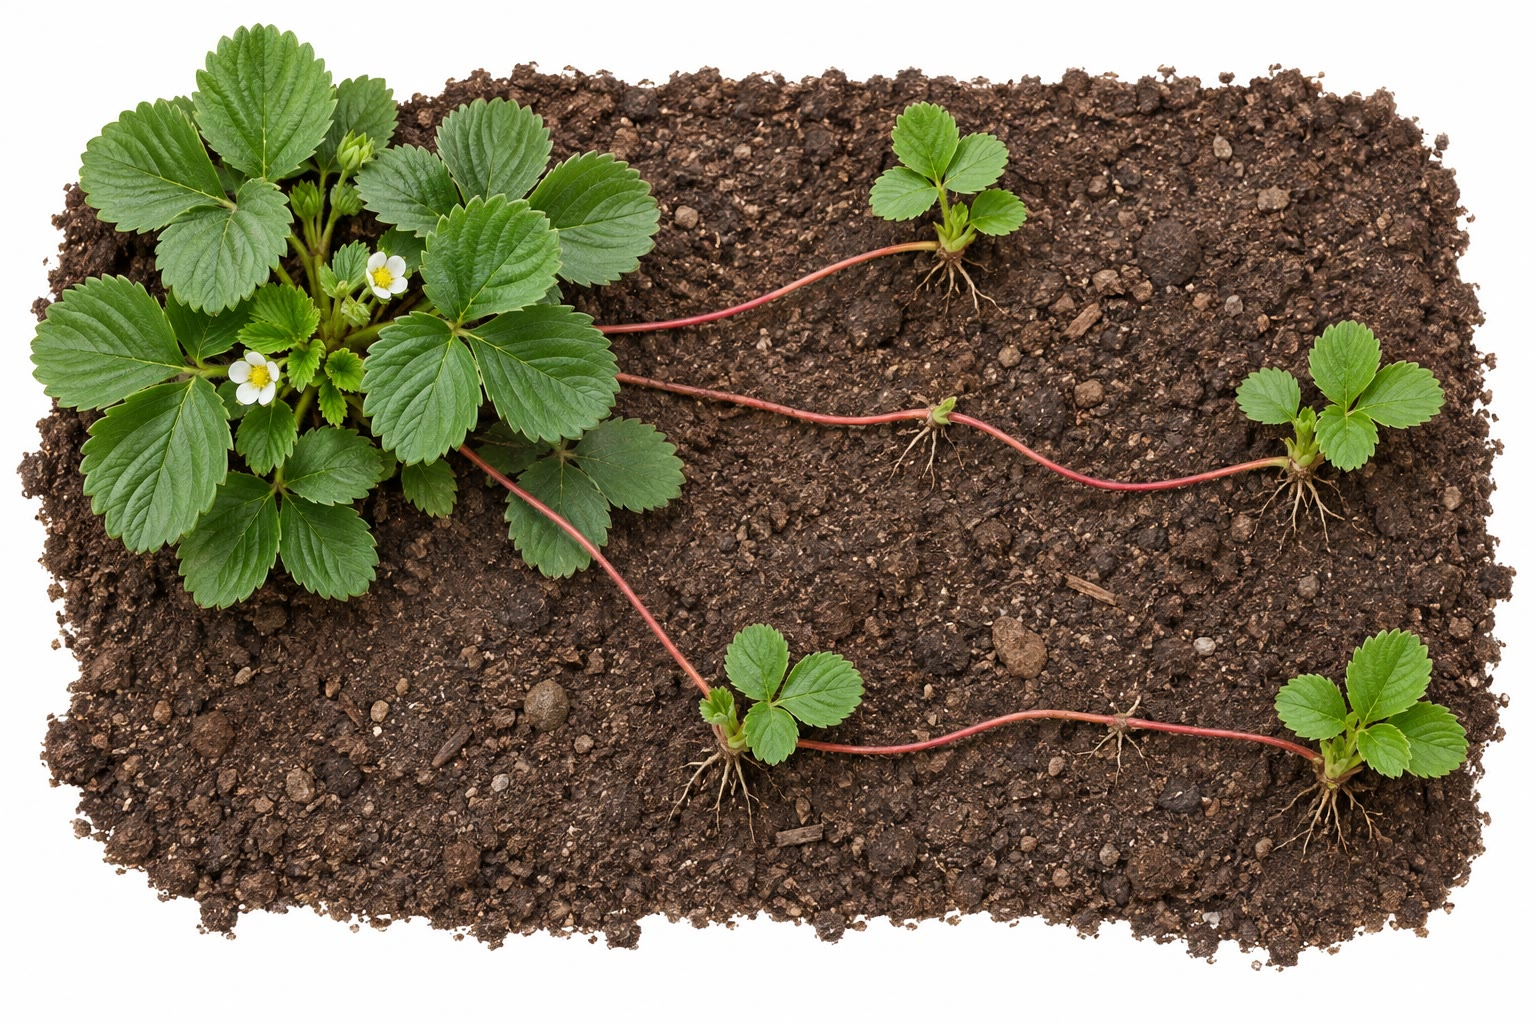
\includegraphics[width=0.46\linewidth]{images/book4/ai/b4-07-strawberry-runners.jpg}\hspace{0.03\linewidth}
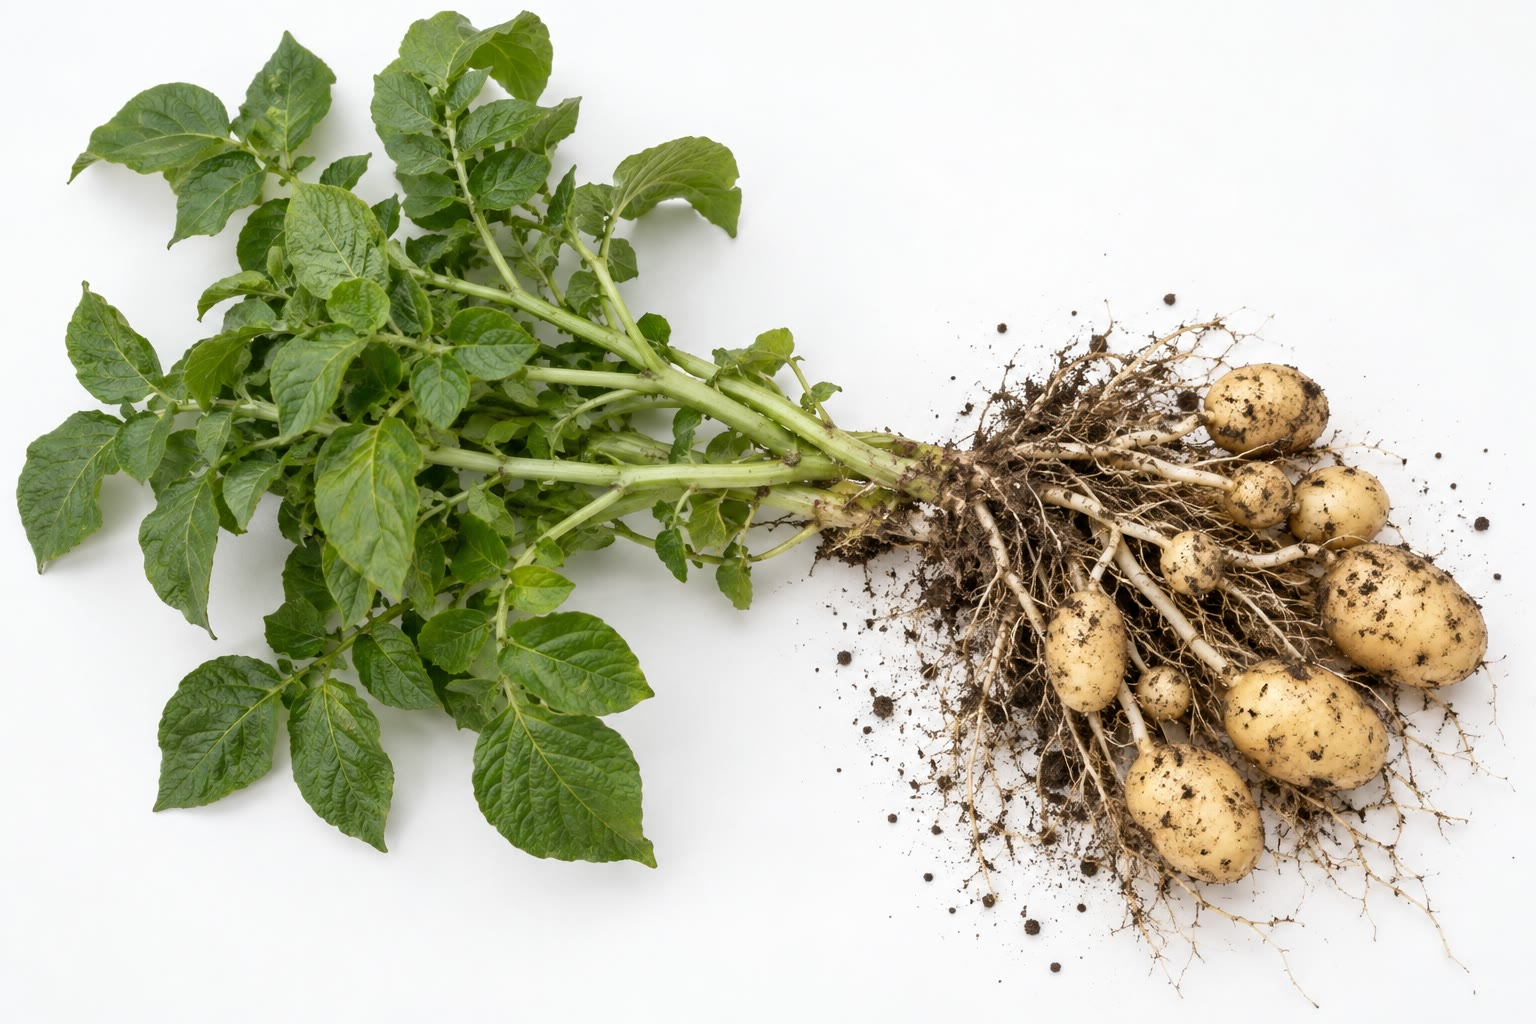
\includegraphics[width=0.46\linewidth]{images/book4/ai/b4-07-potato-tubers.jpg}

{\small बाएँ: कोई स्ट्रॉबेरी पौधा और उसके भूस्तारियों के साथ जड़ पकड़ते
पुत्री-पौधे। दाएँ: मिट्टी से उखाड़ा गया कोई आलू का पौधा, जिसके
कंद स्टोलनों से लटके हैं --- और हर कंद तने का एक टुकड़ा है जो इसी से
आनुवंशिक रूप से समरूप पौधा बनेगा।}
\end{omfigure}

\begin{theorem}[फैलते किसी क्लोन की ज्यामिति]\label{thm:b2:asexual-reproduction:spread}
\index{क्लोनी वृद्धि}
जिस \omterm{def:b2:asexual-reproduction:clone}{जेनेट} का हर \omterm{def:b2:asexual-reproduction:clone}{रैमेट} प्रति वर्ष $m$ जड़ पकड़ी पुत्रियाँ बनाए, और सब
जीवित रहें, उसकी संख्या $N(t) = N_0 (1 + m)^t$ की तरह बढ़ती है --- यानी
बिना किसी लैंगिकता के चरघातांकी वृद्धि --- जब तक \omterm{def:b2:asexual-reproduction:clone}{रैमेट} अपने
वहन-घनत्व $d$ (प्रति इकाई क्षेत्रफल \omterm{def:b2:asexual-reproduction:clone}{रैमेट}) पर जगह न भर लें, जिसके बाद
वह \omterm{def:b2:asexual-reproduction:clone}{क्लोन} एक अग्रिम मोर्चे की तरह आगे बढ़ता है। जो \omterm{def:b2:asexual-reproduction:clone}{क्लोन} अपने भूस्तारी
सीधी रेखा में $v$ चाल से फैलाए उसकी $t$ वर्ष बाद त्रिज्या $vt$ है, और
\omterm{def:b2:asexual-reproduction:clone}{रैमेटों} की संख्या $\pi d (vt)^2$ की तरह बढ़ती है: यानी द्विघातीय रूप से,
चरघातांकी रूप से नहीं। जो स्ट्रॉबेरी पौधा प्रति वर्ष \qty{0.5}{m}
भूस्तारी भेजे उसकी दस वर्ष बाद त्रिज्या \qty{5}{m} है; और आरंभिक
अनुच्छेद का \qty{43}{ha} का ऐस्पन \omterm{def:b2:asexual-reproduction:clone}{क्लोन} कोई \qty{370}{m} त्रिज्या का है
और, प्रति वर्ष कुछ सेंटीमीटर की शुद्ध बढ़त पर, $10^{4}$ वर्ष की कोटि का
पुराना --- जो हिमनदों के पीछे हटने से आँकी गई आयु के अनुरूप है।
\end{theorem}
\begin{proof}
हर वर्ष हर \omterm{def:b2:asexual-reproduction:clone}{रैमेट} की जगह वह स्वयं और $m$ पुत्रियाँ आ जाती हैं, यानी
$1 + m$ का गुणक; और $t$ वर्ष $(1 + m)^t$ देते हैं। भीतर भर जाने के बाद
केवल किनारे के \omterm{def:b2:asexual-reproduction:clone}{रैमेटों} को ही जगह मिलती है, और वह किनारा
भूस्तारी की चाल $v$ से आगे बढ़ता है; क्षेत्रफल $\pi(vt)^2$ है और
\omterm{def:b2:asexual-reproduction:clone}{रैमेटों} की संख्या क्षेत्रफल गुणा घनत्व।
\end{proof}

\begin{example}[सबसे पुराने जीव]\label{ex:b2:asexual-reproduction:oldest}
ऐस्पन \omterm{def:b2:asexual-reproduction:clone}{क्लोन} पांडो (यूटा) \qty{43}{ha} पर लगभग
\num{47000} तनों सहित फैला है, और हर तना कोई सौ वर्ष जीता है तथा उन्हीं
जड़ों के मूल-प्ररोहों से बदल दिया जाता है; वह \omterm{def:b2:asexual-reproduction:clone}{जेनेट} दस हज़ार
वर्ष से भी पुराना हो सकता है। भूमध्यसागर में समुद्री घास
\emph{Posidonia} का कोई \omterm{def:b2:asexual-reproduction:clone}{क्लोन} \qty{15}{km} तक फैला है और लाख वर्ष
पुराना हो सकता है; और मोजावे में क्रिओसोट झाड़ी का एक वलय
\num{11700} वर्ष का आँका गया है, जिसके बीच के तने वलय के फैलने के साथ
मरते जाते हैं। हर स्थिति में जो पुराना है वह \omterm{def:b2:asexual-reproduction:clone}{जेनेट} है; उसकी कोई कोशिका
कुछ दशकों से पुरानी नहीं, और वह जीनोम हज़ारों बार नक़ल हो चुका है।
\end{example}

\section{बिना लैंगिकता के बीज, और बिना पिता के प्राणी}

\begin{definition}[असंगजनन]\label{def:b2:asexual-reproduction:apomixis}
\index{असंगजनन}\index{अनिषेकजनन}
\emph{असंगजनन} बिना निषेचन के \omterm{def:b2:angiosperm-reproduction:seed}{बीज} बनाना है: कोई भ्रूण किसी
अन्यूनित अंडाणु-कोशिका से (\omterm{def:b2:plant-life-cycles:heterospory}{गुरुबीजाणु} की मातृ कोशिका
\omterm{def:b2:meiosis-heredity:meiosis}{अर्धसूत्री विभाजन} छोड़ देती है) या सीधे बीजांडकाय की किसी कोशिका से
विकसित होता है, और वह \omterm{def:b2:angiosperm-reproduction:seed}{बीज} माता का \omterm{def:b2:meiosis-heredity:vocabulary}{जीन-प्ररूप} ढोता है। डैंडेलायन, हॉकवीड,
ब्लैकबेरी, केंटकी ब्लूग्रास और अनेक सिट्रस ऐसा करते हैं; और सिट्रस का
\omterm{def:b2:angiosperm-reproduction:seed}{बीज} प्रायः कई भ्रूण रखता है, एक लैंगिक और बाक़ी माता की
बीजांडकायी प्रतियाँ। असंगजनन \omterm{def:b2:angiosperm-reproduction:seed}{बीज} को --- उसके प्रकीर्णन, \omterm{def:b2:angiosperm-reproduction:seed}{प्रसुप्ति} और
आवरण को --- रख लेता है और \omterm{def:b2:meiosis-heredity:meiosis}{अर्धसूत्री विभाजन} छोड़ देता है, इसलिए कोई
भली-भाँति अनुकूलित \omterm{def:b2:meiosis-heredity:vocabulary}{जीन-प्ररूप} अपरिवर्तित प्रसारित हो जाता है; और
अधिकांश असंगजनक संकर उद्गम के \omterm{def:b2:genome-diversification:polyploidy}{बहुगुणित} हैं जिनका
\omterm{def:b2:meiosis-heredity:meiosis}{अर्धसूत्री विभाजन} वैसे भी विफल हो जाता। प्राणियों में इसका समकक्ष
\emph{अनिषेकजनन} है, यानी किसी अनिषेचित अंडाणु से विकास:
कुछ छिपकलियों में और ब्डेलॉइड रोटिफ़रों में अनिवार्य, जिनमें करोड़ों
वर्षों से कोई नर नहीं रहा; और माहू तथा जल-पिस्सुओं में चक्रीय, जो पूरी
गर्मी अनिषेकजनन से गुणित होते हैं, और कोई मादा ऐसी जीवित पुत्रियों को
जन्म देती है जो पहले से अपने भ्रूण ढोती हैं, और शरद में किसी लैंगिक
पीढ़ी पर चले जाते हैं जो शीतकाल पार करने वाले अंडे देती है।
\end{definition}

\begin{omfigure}
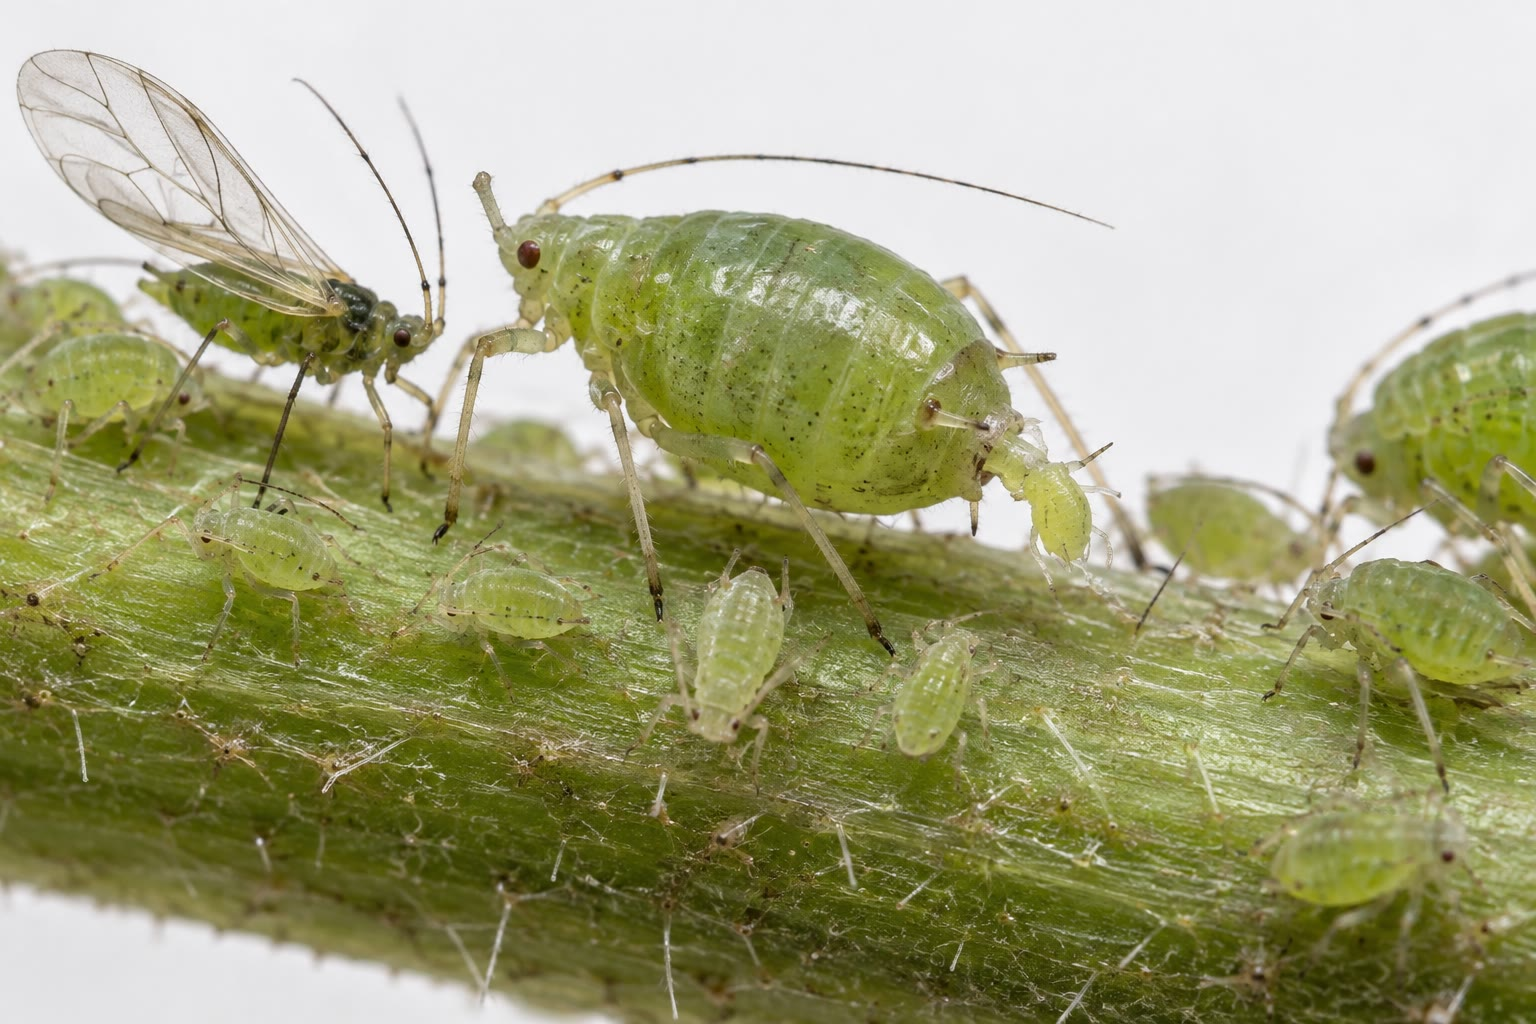
\includegraphics[width=0.55\linewidth]{images/book4/ai/b4-07-aphids.jpg}

{\small किसी तने पर माहू: एक पंखहीन अनिषेकजनक मादा एक जीवित पुत्री को
जन्म देती हुई, कई आयुओं की निम्फ़, और एक पंखदार
प्रवासी --- यानी एक भी नर के बिना एक ग्रीष्म की चरघातांकी वृद्धि।}
\end{omfigure}

\begin{example}[माहू की एक गर्मी]\label{ex:b2:asexual-reproduction:aphids}
कोई अनिषेकजनक माहू लगभग आठ दिन में परिपक्व होती है और दो सप्ताह तक
प्रतिदिन कोई पाँच पुत्रियाँ देती है; और वे पुत्रियाँ पहले से गर्भवती
जन्म लेती हैं (भ्रूण माता के भ्रूणों के भीतर ही विकसित होने लगते हैं)।
दस दिन के पास के \omterm{def:b2:unicellular-diversity:division}{पीढ़ी काल} और प्रति पीढ़ी लगभग \num{50} की
शुद्ध वृद्धि दर के साथ, अप्रैल की एक अकेली संस्थापक, बिना रोक-टोक,
चार महीनों के भीतर $50^{12} \approx 2\times 10^{20}$ संतति छोड़
देती --- यानी आज जीवित हर प्राणी से अधिक द्रव्यमान। गुबरैले, लेसविंग,
परजीवी ततैया, कवक और वर्षा उस संख्या को प्रति पौधा कुछ हज़ार तक रखते
हैं, और शरद की लैंगिक पीढ़ी सर्दी से पहले उस \omterm{def:b2:asexual-reproduction:clone}{क्लोन} को
पुनर्संयोजित अंडों में फिर से बाँट देती है।
\end{example}

\section{उगाने वाले का क्लोनन}

\begin{proposition}[कलम, दाबन, ग्राफ़्टिंग]\label{prop:b2:asexual-reproduction:horticulture}
\index{कलम}\index{ग्राफ़्टिंग}\index{मूलवृंत}
\emph{कलम} तने, जड़ या पत्ती का ऐसा टुकड़ा है जिसे जड़ पकड़ने को प्रेरित
किया जाए: कटे सिरे पर विभाजित होती कोशिकाओं का कैलस बनता है जिससे मूल
विभज्योतक उठते हैं, और इसमें ऑक्सिन (जड़ लगाने वाला हॉर्मोन) तथा आर्द्रता
सहायक होते हैं। \emph{दाबन} किसी शाखा को जुड़े रहते हुए जड़ पकड़ाता है
और बाद में काट देता है। \emph{ग्राफ़्टिंग} किसी एक पौधे के प्ररोह (यानी
\emph{कलिकाग्र}) को किसी दूसरे के जड़दार तने (यानी \emph{मूलवृंत}) से
जोड़ती है: दोनों कैंबियम दबाकर मिलाए जाते हैं, कैलस घाव पर पुल बनाता है,
और सप्ताहों के भीतर नया जाइलम तथा फ्लोएम उसके आरपार जुड़ जाते हैं। वह
ग्राफ़्ट एक काइमेरा है --- जड़ें मूलवृंत का जीनोम रखती हैं और फलदार
प्ररोह कलिकाग्र का --- और वह केवल सगे पौधों के बीच चलती है (एक ही वंश
की, कभी-कभी एक ही कुल की जातियाँ), क्योंकि ऊतकों को एक-दूसरे की कोशिकाएँ
पहचाननी पड़ती हैं। सेब, नाशपाती, चेरी, सिट्रस और अंगूर की हर क़िस्म
ग्राफ़्टिंग से प्रवर्धित होती है: कोई नामित क़िस्म एक ही
\omterm{def:b2:asexual-reproduction:clone}{जेनेट} है, जिसे कलिकाग्रों से सदियों जीवित रखा गया है (रेनेट सेब सोलहवीं
शताब्दी के हैं), और मूलवृंत मिट्टी, रोग और चाहे गए वृक्ष-आकार के अनुसार
चुना जाता है --- बौनाकारी मूलवृंत ही आधुनिक बग़ीचों के छोटे वृक्ष
बनाते हैं।
\end{proposition}

\begin{proposition}[सूक्ष्मप्रवर्धन और पूर्णशक्तता]\label{prop:b2:asexual-reproduction:tissueculture}
\index{सूक्ष्मप्रवर्धन}\index{पूर्णशक्तता}\index{कैलस}
केंद्रक वाली कोई भी जीवित पादप कोशिका, सिद्धांततः, पूरा पौधा फिर से गढ़
सकती है। \emph{ऊतक संवर्धन} में ऊतक का कोई निर्जीवाणुकृत टुकड़ा
(कोई \emph{बहिर्भाग}: कोई प्ररोह-शीर्ष, कोई पर्ण-चक्रिका, कोई परागकोश)
शर्करा, खनिज, विटामिन और हॉर्मोन वाले किसी अगार माध्यम पर रखा जाता है।
ऑक्सिन और साइटोकाइनिन संतुलन में हों तो कोशिकाएँ विभेदन खोकर
\emph{कैलस} बन जाती हैं, यानी विभाजित होती अविशिष्ट कोशिकाओं का पिंड;
ऑक्सिन से अधिक साइटोकाइनिन हो तो कैलस प्ररोह बनाता है, साइटोकाइनिन से
अधिक ऑक्सिन हो तो जड़ें, और कुछ जातियों में वह \emph{कायिक
भ्रूण} बनाता है --- यानी बिना किसी अंडाणु के पूरे भ्रूण। प्ररोह हर कुछ
सप्ताह में काटकर उपसंवर्धित किए जाते हैं और हर बार तीन से
दस गुना हो जाते हैं, इसलिए एक विभज्योतक एक वर्ष में दस लाख पौधक देता
है। चूँकि विषाणु बढ़ते शीर्ष से पीछे रह जाते हैं, इसलिए किसी संक्रमित
पौधे में भी एक मिलिमीटर से छोटा प्ररोह-विभज्योतक प्रायः विषाणु-मुक्त
होता है: \emph{विभज्योतक संवर्धन} से ही आलू, स्ट्रॉबेरी, केला और
ऑर्किड के भंडार साफ़ किए जाते हैं। यह विधि पूर्णशक्तता का
व्यावहारिक प्रमाण है, और वही कारण कि कोई पादप क़िस्म अपने सृजन के कुछ ही
वर्षों में लाखों की संख्या में बेची जा सकती है।
\end{proposition}
\begin{proof}[प्रमाण-सामग्री]
स्कूग और मिलर (1957) ने तंबाकू के मज्जा-कैलस को ऑक्सिन तथा नई खोजी गई
साइटोकाइनिन के भिन्न अनुपातों वाले माध्यमों पर उगाया: अधिक
ऑक्सिन ने जड़ें दीं, अधिक साइटोकाइनिन ने प्ररोह, और संतुलन ने केवल
कैलस --- यानी अंग-निर्माण दो हॉर्मोनों के अनुपात से तय था, किसी
विशिष्ट अंग-कारक पदार्थ से नहीं। स्टीवर्ड (1958) ने किसी गाजर की जड़ की
अकेली कोशिकाएँ और छोटे गुच्छे नारियल-पानी के घूमते फ़्लास्क में निलंबित
किए: कुछ गुच्छों ने भ्रूण जैसी संरचनाएँ बनाईं जो बढ़कर पूरी फूलती हुई
गाजरें बन गईं, और यों दिखाया कि किसी परिपक्व अंग की कोई विभेदित
कोशिका विकास का पूरा कार्यक्रम अब भी रखती है और काम में ले सकती है।
\end{proof}

\begin{omfigure}
\begin{tikzpicture}[every node/.style={font=\scriptsize}, >=stealth]
  \node[draw, rounded corners, fill=omDef!12, align=center] (ex) at (0,0) {बहिर्भाग\\(प्ररोह-शीर्ष, पर्ण-चक्रिका)};
  \node[draw, rounded corners, fill=omExo!30, align=center] (cal) at (4.6,0) {कैलस\\ऑक्सिन $\approx$ साइटोकाइनिन};
  \node[draw, rounded corners, fill=omExo!30, align=center] (sh) at (8.4,1.2) {प्ररोह\\साइटोकाइनिन $>$ ऑक्सिन};
  \node[draw, rounded corners, fill=omExo!30, align=center] (rt) at (8.4,-1.2) {जड़ें\\ऑक्सिन $>$ साइटोकाइनिन};
  \node[draw, rounded corners, fill=omDef!12, align=center] (pl) at (12.2,0) {पौधक\\मिट्टी में अभ्यस्त किए हुए};
  \draw[->, thick] (ex) -- (cal) node[midway, below, align=center] {निर्जीवाणु\\माध्यम};
  \draw[->, thick] (cal) -- (sh); \draw[->, thick] (cal) -- (rt);
  \draw[->, thick] (sh) -- (pl); \draw[->, thick] (rt) -- (pl);
  \draw[->, thick, omThm] (sh) .. controls (8.4,2.6) and (5.8,2.6) .. (5.2,0.6);
  \node[omThm, anchor=south] at (6.9,2.3) {हर 4 सप्ताह उपसंवर्धन, $\times 5$};
\end{tikzpicture}

{\small सूक्ष्मप्रवर्धन: किसी बहिर्भाग को विभेदन खोकर
कैलस बनाया जाता है, ऑक्सिन-साइटोकाइनिन अनुपात से उसे प्ररोहों या जड़ों
की ओर मोड़ा जाता है, और पौधकों को मिट्टी में अभ्यस्त करने से पहले
बार-बार उपसंवर्धन से गुणित किया जाता है।}
\end{omfigure}

\begin{omfigure}
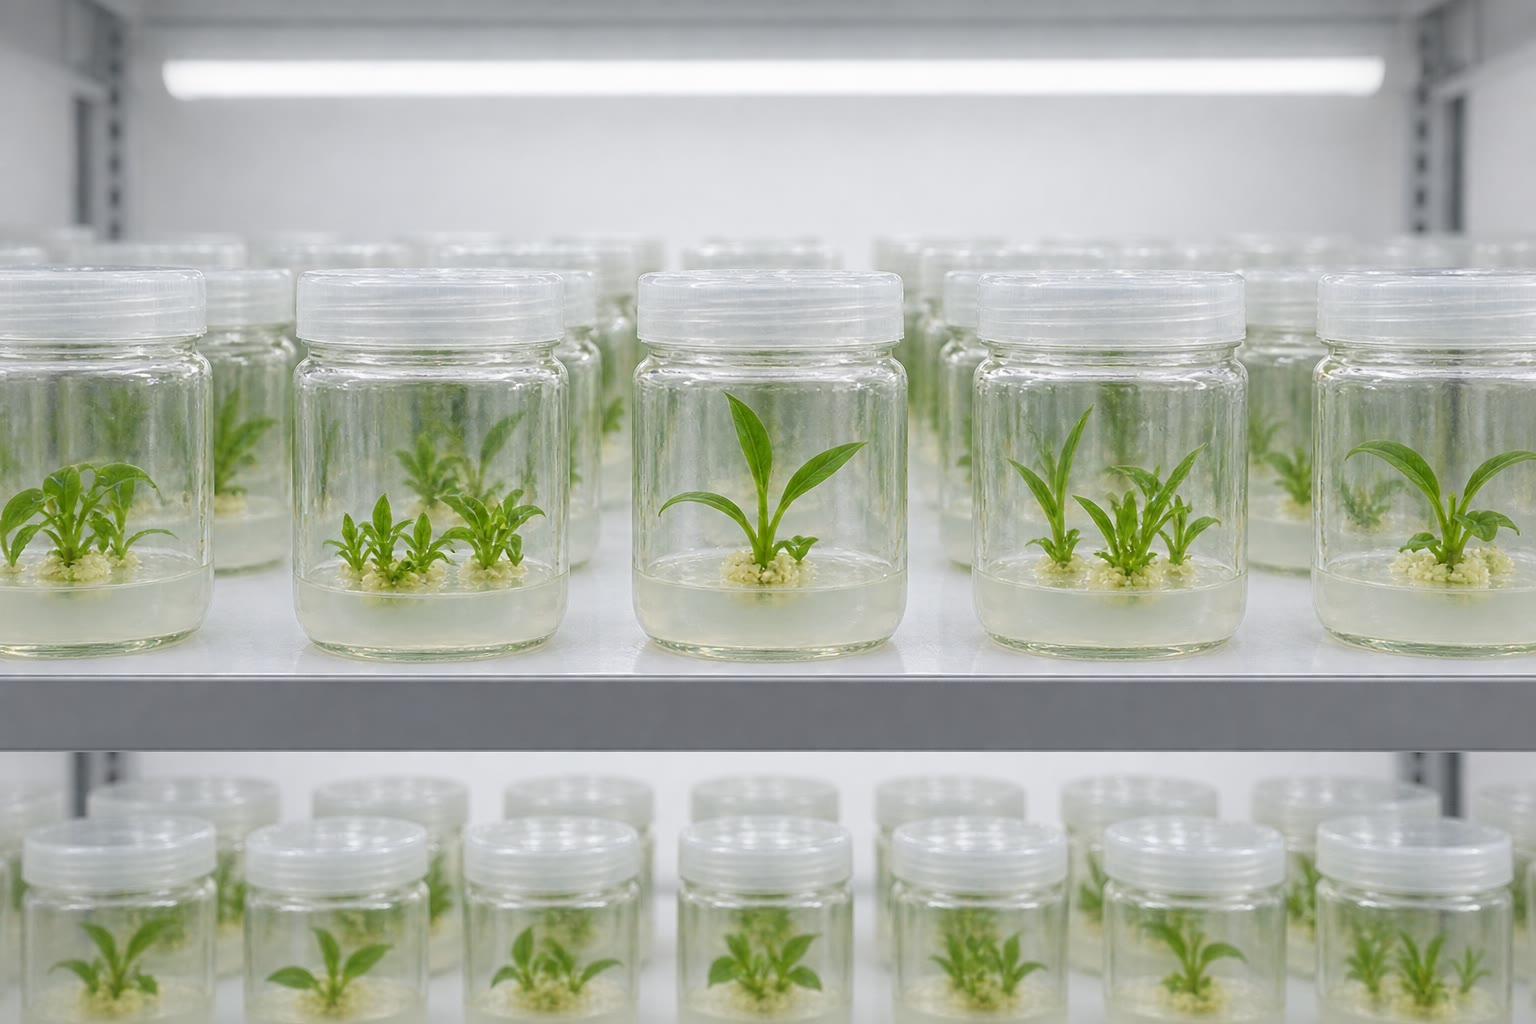
\includegraphics[width=0.6\linewidth]{images/book4/ai/b4-07-tissue-culture.jpg}

{\small किसी वृद्धि-कक्ष में अगार पर पौधक: हर मर्तबान उसी क़िस्म का एक
\omterm{def:b2:asexual-reproduction:clone}{क्लोन} रखता है, जो किसी एक विभज्योतक से गुणित हुआ है।}
\end{omfigure}

\section{लैंगिकता का दाम और उसके बिना रहने का दाम}

\begin{theorem}[लैंगिकता का दुगुना दाम]\label{thm:b2:asexual-reproduction:twofold}
\index{लैंगिकता का दुगुना दाम}
जिस आबादी में हर मादा $F$ संतान बनाती हो, जिनमें से आधे पुत्र हों, वहाँ
कोई अलैंगिक उत्परिवर्ती मादा, जो $F$ पुत्रियाँ बनाती है और सब अपनी ही
प्रतियाँ, अगली पीढ़ी की मादाओं में अपना हिस्सा दुगुना कर लेती है।
यदि उस अलैंगिक वंशक्रम की बारंबारता मादाओं में $p$ हो, तो अगली पीढ़ी में
\[
p' = \frac{2p}{1 + p}, \qquad p_t = \frac{2^t p_0}{1 + (2^t - 1)p_0},
\]
यानी एक हज़ार में एक से चलकर वह दस पीढ़ियों में आधी आबादी तक और उसके
कुछ ही बाद पूरी तक पहुँच जाता है। बाक़ी सब बराबर हो तो
लैंगिकता किसी वंशक्रम के गुणित होने की दर आधी कर देती है --- यही नर
बनाने का दाम है। और चूँकि लैंगिकता फिर भी लगभग सार्वभौम है, इसलिए बाक़ी
सब बराबर नहीं है: लैंगिक वंशक्रमों को पुनर्संयोजन से, औसतन, कम से कम दो
का गुणक मिलना ही चाहिए।
\end{theorem}
\begin{proof}
अलैंगिक मादाएँ $pN$ हैं और $FpN$ पुत्रियाँ छोड़ती हैं; लैंगिक
मादाएँ $(1 - p)N$ हैं और $F(1 - p)N/2$ पुत्रियाँ छोड़ती हैं (बाक़ी
आधे पुत्र हैं, जो कोई अंडाणु नहीं बनाते)। पुत्रियों में अलैंगिक हिस्सा
$Fp/(Fp + F(1 - p)/2) = 2p/(1 + p)$ है। $q = p/(1 -
p)$ लिखने पर वह पुनरावृत्ति $q' = 2q$ हो जाती है, इसलिए $q_t = 2^t q_0$;
और वापस बदलने पर $p_t$ मिलता है। $p_t = \tfrac12$ रखने पर $2^t q_0 = 1$, यानी
$t = \log_2(1/q_0) \approx 10$ जब $p_0 = 10^{-3}$।
\end{proof}

\begin{omfigure}
\begin{tikzpicture}
\begin{axis}[
  width=0.76\linewidth, height=5.6cm,
  axis x line=bottom, axis y line=left,
  xmin=0, xmax=20, ymin=0, ymax=1.05,
  xlabel={पीढ़ियाँ}, ylabel={अलैंगिक वंशक्रम की बारंबारता},
  xlabel style={font=\small, at={(axis description cs:0.5,-0.13)}, anchor=north},
  ylabel style={font=\small},
  tick label style={font=\small}, xtick={0,5,10,15,20}, ytick={0,0.5,1},
  legend style={font=\scriptsize, at={(0.5,-0.3)}, anchor=north, draw=none},
  clip=false,
]
\addplot[very thick, omThm, domain=0:20, samples=80] {2^x*0.001/(1+(2^x-1)*0.001)};
\addlegendentry{और कोई अंतर नहीं: 12 पीढ़ियों में छा जाता है}
\addplot[very thick, omDef, domain=0:20, samples=80] {0.001*(1.3)^x/(1+(1.3^x-1)*0.001)};
\addlegendentry{अलैंगिक परजीवियों से \qty{35}{\%} सुयोग्यता खोते हैं: धीमा}
\addplot[very thick, omProp, domain=0:20, samples=80] {0.001*(0.9)^x/(1+(0.9^x-1)*0.001)};
\addlegendentry{अलैंगिक \qty{55}{\%} खोते हैं: वे कभी नहीं फैलते}
\end{axis}
\end{tikzpicture}

{\small दुगुना लाभ क्रिया में। एक हज़ार में एक से आरंभ करके, जिस
अलैंगिक वंशक्रम को और कोई हानि न हो वह एक दर्जन पीढ़ियों में छा जाता
है; और उसे केवल आधे से अधिक की सुयोग्यता-हानि ही रोक पाती है ---
परजीवियों से, जमा होते \omterm{def:b2:genome-diversification:mutation}{उत्परिवर्तनों} से, या धीमे अनुकूलन से।}
\end{omfigure}

\begin{proposition}[लैंगिकता किसलिए है]\label{prop:b2:asexual-reproduction:whysex}
\index{मुलर का रैचट}\index{लाल रानी परिकल्पना}
तीन लाभ इतने बड़े हैं कि मायने रखें। \emph{\omterm{prop:b2:asexual-reproduction:whysex}{मुलर का रैचट}}:
किसी \omterm{def:b2:asexual-reproduction:clone}{क्लोन} में हर हानिकारक \omterm{def:b2:genome-diversification:mutation}{उत्परिवर्तन} सारी संतति को विरासत में मिलता
है, और जो उत्परिवर्तन-मुक्त जीनोम किसी परिमित आबादी से एक बार संयोग से
खो जाए वह कभी फिर नहीं गढ़ा जा सकता; वह बोझ एक-एक खटके से ऊपर चढ़ता जाता
है, और छोटी अलैंगिक आबादियाँ क्षीण हो जाती हैं। पुनर्संयोजन दो
क्षतिग्रस्त जीनोमों से स्वच्छ जीनोम फिर गढ़ देता है। \emph{अनुकूलन}: किसी
\omterm{def:b2:asexual-reproduction:clone}{क्लोन} के भिन्न व्यक्तियों में उठे दो उपयोगी \omterm{def:b2:genome-diversification:mutation}{उत्परिवर्तन} होड़ करते हैं और
एक खो जाता है; किसी लैंगिक आबादी में वे जुड़ जाते हैं (फ़िशर और मुलर,
1930 का दशक), इसलिए जब अनेक जीन बदलने हों तब लैंगिक आबादियाँ तेज़
अनुकूलित होती हैं। \emph{लाल रानी}: परजीवी सबसे आम पोषी
\omterm{def:b2:meiosis-heredity:vocabulary}{जीन-प्ररूप} के अनुरूप ढल जाते हैं, और कोई \omterm{def:b2:asexual-reproduction:clone}{क्लोन}, एक ही \omterm{def:b2:meiosis-heredity:vocabulary}{जीन-प्ररूप} होने से,
सबसे आम है; जबकि लैंगिक जनक हर संतान को एक नया ताला बना देते हैं। जिन
घोंघों, मछलियों और पौधों की लैंगिक तथा क्लोनी दोनों आबादियाँ हैं उनमें
लैंगिक आबादियाँ वहीं जीतती दिखती हैं जहाँ परजीवी प्रचुर हैं। जो अलैंगिक
वंशक्रम फल-फूल रहे हैं --- डैंडेलायन, ब्डेलॉइड रोटिफ़र, अधिकांश फ़सली
\omterm{def:b2:asexual-reproduction:clone}{क्लोन} --- वे या तो नए हैं, या \omterm{def:b2:genome-diversification:polyploidy}{बहुगुणित} संकर हैं जो अपनी ही
विविधता ढोते हैं, या किसी उगाने वाले के सहारे टिके हैं जो उनके परजीवी
उनके लिए मार देता है।
\end{proposition}

\begin{example}[किसी क्लोन के एकशस्य]\label{ex:b2:asexual-reproduction:monoculture}
1840 के दशक में आयरलैंड की अधिकांश आलू-फ़सल एक ही क्लोनी
क़िस्म, लंपर, थी; और 1845 में आया जल-फफूँद \emph{Phytophthora infestans}
ऐसे देश से मिला जहाँ पौधे आनुवंशिक रूप से समरूप और एक जैसे
सुग्राही थे, और उसने लगातार तीन वर्ष वह फ़सल नष्ट कर दी।
1950 के दशक तक विश्व का निर्यात-केला एक ही \omterm{def:b2:asexual-reproduction:clone}{क्लोन} था, ग्रो
मिशेल, जिसे किसी मृदा-कवक ने मध्य अमेरिकी बाग़ानों से मिटा दिया;
उसका स्थान लेने वाला कैवेंडिश भी एक ही \omterm{def:b2:asexual-reproduction:clone}{क्लोन} है और अब उसी कवक के एक नए
विभेद से, बाग़ान-दर-बाग़ान, खोया जा रहा है, जिसके सामने उसके पास कोई
विविधता नहीं है। कोई \omterm{def:b2:asexual-reproduction:clone}{क्लोन} प्रकृति का सबसे आसान निशाना है,
और जो उगाने वाला उसे बोता है उसे वह प्रतिरोध स्वयं जुटाना पड़ता है जो
पुनर्संयोजन मुफ़्त में जुटा देता।
\end{example}

\section{अभ्यास}

\begin{exercise}[$\star$]\label{exo:b2:asexual-reproduction:1}
\omterm{def:b2:asexual-reproduction:clone}{क्लोन}, \omterm{def:b2:asexual-reproduction:clone}{जेनेट} और \omterm{def:b2:asexual-reproduction:clone}{रैमेट} की परिभाषा दीजिए, और
\omterm{def:b2:asexual-reproduction:clone}{कायिक गुणन} के तीन प्राकृतिक अंग बताइए, हर एक के लिए एक पौधा देते हुए।
\end{exercise}

\begin{exercise}[$\star$]\label{exo:b2:asexual-reproduction:2}
किसी ग्राफ़्ट में संधि के सफल होने के लिए किन ऊतकों का मिलना आवश्यक है,
और हर साथी वृक्ष को क्या देता है? कोई ग्राफ़्ट किया वृक्ष काइमेरा क्यों
है और संकर क्यों नहीं?
\end{exercise}

\begin{exercise}[$\star$]\label{exo:b2:asexual-reproduction:3}
\omterm{def:b2:asexual-reproduction:apomixis}{असंगजनन} और \omterm{def:b2:asexual-reproduction:clone}{कायिक गुणन} में भेद कीजिए, तथा
\omterm{def:b2:asexual-reproduction:apomixis}{अनिषेकजनन} को दोनों से अलग कीजिए। इन तीनों में से कौन \omterm{def:b2:angiosperm-reproduction:seed}{बीज} रखता है?
\end{exercise}

\begin{exercise}[$\star$]\label{exo:b2:asexual-reproduction:4}
बहिर्भाग से लेकर खेत के पौधे तक सूक्ष्मप्रवर्धन के चरण बताइए, और हर एक
पर हॉर्मोन-परिस्थितियाँ नामित कीजिए।
\end{exercise}

\begin{exercise}[$\star\star$]\label{exo:b2:asexual-reproduction:5}
कोई स्ट्रॉबेरी पौधा प्रति वर्ष 8 भूस्तारी बनाता है, और हर एक 3
पौधक जड़ पकड़ाता है, और हर पौधक अगले वर्ष वही करता है।
कोई न मरे तो 4 वर्ष बाद कितने पौधे? प्रति पौधा \qty{0.1}{m^2} पर
उन्हें कितना क्षेत्रफल चाहिए? उस \omterm{def:b2:asexual-reproduction:clone}{क्लोन} को असल में क्या सीमित करता है?
\end{exercise}

\begin{exercise}[$\star\star$]\label{exo:b2:asexual-reproduction:6}
ऐस्पन \omterm{def:b2:asexual-reproduction:clone}{क्लोन} पांडो के \qty{43}{ha} पर \num{47000} तने हैं, और हर
तना लगभग \num{130} वर्ष जीता है। यदि वह \omterm{def:b2:asexual-reproduction:clone}{जेनेट} \num{14000} वर्ष
पुराना हो, तो उसकी कितनी तना-पीढ़ियाँ हो चुकी हैं? उसे चक्रिका मानकर
उसकी माध्य त्रिज्य बढ़त मीटर प्रति वर्ष में निकालिए।
\end{exercise}

\begin{exercise}[$\star\star$]\label{exo:b2:asexual-reproduction:7}
किसी लैंगिक आबादी में $10^{-4}$ बारंबारता पर उतनी ही उर्वरता वाला कोई
अलैंगिक उत्परिवर्ती उठता है। 5,
10 और 15 पीढ़ियों बाद उसकी बारंबारता निकालिए। उसके कभी न फैलने के लिए
उसकी सुयोग्यता कितनी घटनी चाहिए?
\end{exercise}

\begin{exercise}[$\star\star$]\label{exo:b2:asexual-reproduction:8}
भविष्यवाणी कीजिए कि तंबाकू का कोई कैलस ऑक्सिन : साइटोकाइनिन
अनुपात 10 : 1, 1 : 1 और 1 : 10 वाले माध्यमों पर क्या करता है, और
समझाइए कि किसी प्ररोह-कलम को ऑक्सिन में क्यों डुबोया जाता है, साइटोकाइनिन में क्यों नहीं।
\end{exercise}

\begin{exercise}[$\star\star$]\label{exo:b2:asexual-reproduction:9}
आलू कंदों के रूप में बोए जाते हैं। बोया गया एक किलोग्राम
\qty{10}{kg} देता है, और एक हेक्टेयर को \qty{2}{t} बीज-कंद चाहिए। किसी
नई क़िस्म के \qty{1}{kg} से आरंभ करके, एक हेक्टेयर बोने में कितनी ऋतुएँ
लगेंगी? असली \omterm{def:b2:angiosperm-reproduction:seed}{बीज} तेज़ गुणन क्यों देता है पर काम में क्यों नहीं लिया
जाता?
\end{exercise}

\begin{exercise}[$\star\star\star$]\label{exo:b2:asexual-reproduction:10}
$N$ व्यक्तियों की किसी क्लोनी आबादी में, जिसमें प्रति जीनोम प्रति पीढ़ी
$U$ हानिकारक \omterm{def:b2:genome-diversification:mutation}{उत्परिवर्तन} हों और हर एक सुयोग्यता का अंश $s$ लेता हो,
साम्य पर उत्परिवर्तन-मुक्त व्यक्तियों का अंश
$e^{-U/s}$ है (\cref{ch:b2:population-genetics} में व्युत्पन्न)। $U =
0.1$ और $s = 0.02$ के साथ $N = 10^{5}$ तथा $N = 10^{3}$ के लिए
उत्परिवर्तन-मुक्त व्यक्तियों की संख्या निकालिए, और
मुलर के रैचट से समझाइए कि छोटी आबादी क्यों डूबी हुई है और बड़ी
क्यों नहीं --- अभी नहीं।
\end{exercise}

\begin{exercise}[$\star\star\star$]\label{exo:b2:asexual-reproduction:11}
किसी दिए हुए \omterm{def:b2:meiosis-heredity:vocabulary}{जीन-प्ररूप} का प्रतिरोध तोड़ देने वाला कोई रोगजनक विभेद
एक बार उठता है। एक ही \omterm{def:b2:asexual-reproduction:clone}{क्लोन} के खेत में और ऐसी किसी
लैंगिक आबादी में, जिसमें प्रतिरोध के जीन दस स्थलों पर पृथक होते हैं और
हर स्थल पर बराबर बारंबारता के दो \omterm{def:b2:meiosis-heredity:vocabulary}{युग्मविकल्पी} हैं, उसकी नियति की तुलना
कीजिए, और आयरलैंड के आलू-अकाल को इन्हीं पदों में समझाइए।
\end{exercise}

\begin{exercise}[$\star\star\star$]\label{exo:b2:asexual-reproduction:12}
``लैंगिकता का दाम दो का गुणक है और वह सर्वत्र है; अलैंगिकता सस्ती है
और विरल।'' अध्याय के तीनों स्पष्टीकरणों पर विचार कीजिए, और बताइए कि
ब्डेलॉइड रोटिफ़र --- चार करोड़ वर्ष से अलैंगिक --- हर एक के लिए
क्या संकेत करते हैं।
\end{exercise}

\section{समस्या: एक स्ट्रॉबेरी फ़ार्म और एक पुराना क्लोन}

\begin{problem}[{सप्तांत समस्या --- किसी क्लोन का अंकगणित, भूस्तारियों
से भरते किसी स्ट्रॉबेरी खेत और किसी विभज्योतक को गुणित करती प्रयोगशाला
से लेकर किसी लैंगिक आबादी पर किसी असंगजनक के आक्रमण और किसी प्राचीन
जेनेट के आनुवंशिक क्षय तक, और अंत खेत भरने के काल, एक विभज्योतक से मिलते
पौधकों, तथा असंगजनकों और लैंगिकों के साम्य पर}]
\label{pb:b2:asexual-reproduction:1}
कोई उगाने वाला \qty{1}{ha} के ऐसे खेत में \num{100} स्ट्रॉबेरी पौधे
बोता है जो प्रति वर्ग मीटर \num{4} पौधे सँभाल सकता है। हर
पौधा प्रति वर्ष \num{6} भूस्तारी बनाता है, और हर भूस्तारी \num{2}
पुत्रियाँ जड़ पकड़ाता है, और सारे पौधे बचे रहते हैं। कोई प्रयोगशाला उसी
क़िस्म को ऊतक संवर्धन से गुणित करती है: हर \num{4} सप्ताह पर हर उपसंवर्धन
प्ररोहों को \num{5} गुना करता है; और \qty{80}{\%} पौधक अभ्यस्तीकरण झेल
जाते हैं। उस क़िस्म की साधारण कलमें \qty{90}{\%} विषाणु-संक्रमित हैं;
और \qty{0.3}{mm} के विभज्योतक शीर्ष $0.02$ प्रायिकता से वह विषाणु ढोते
हैं। ऐस्पन जीनोम: \qty{4.8e8}{} क्षारक युग्म; कायिक \omterm{thm:b2:genome-diversification:rate}{उत्परिवर्तन दर}
प्रति क्षारक युग्म प्रति कोशिका-विभाजन \qty{1e-9}{}; और किसी बढ़ते
प्ररोह में प्रति वर्ष \num{20} विभज्योतक कोशिका-विभाजन।

\medskip
\noindent\textbf{भाग I --- खेत भरना।}
\begin{enumerate}
  \item वह खेत कितने पौधे सँभाल सकता है?
  \item हर वर्ष पौधों की संख्या किस गुणक से बढ़ती है?
  \item 1, 2 और 3 वर्ष बाद पौधों की संख्या निकालिए।
  \item खेत के भर जाने का काल पाने के लिए $N(t) = 100\times 13^{t}$
        हल कीजिए।
  \item भर जाने के बाद केवल किसी खंड के किनारे के पौधों को ही जगह
        मिलती है। यदि कोई खंड प्रति वर्ष \qty{0.5}{m} आगे बढ़े, तो
        केवल बढ़त से पूरा खेत ढकने में एक पौधे को कितने वर्ष लगते?
  \item समझाइए कि वह उगाने वाला एक पौधे के बजाय खेत भर में फैलाकर
        \num{100} पौधे क्यों बोता है।
\end{enumerate}

\medskip
\noindent\textbf{भाग II --- प्रयोगशाला।}
\begin{enumerate}[resume]
  \item एक विभज्योतक से कम से कम $10^{6}$ प्ररोह तक जाने के लिए कितने
        उपसंवर्धन चाहिए? कितने सप्ताह?
  \item अभ्यस्तीकरण के बाद कितने पौधे बचते हैं?
  \item किसी विभज्योतक-जनित वंशक्रम के विषाणु-मुक्त होने की प्रायिकता
        क्या है? और एक ही पौधे से आरंभ की गई सारी \num{10} वंशक्रमों के
        होने की?
  \item वह प्रयोगशाला \num{10} वंशक्रम आरंभ करती है और जाँच के बाद
        संक्रमित वंशक्रम फेंक देती है। स्वच्छ वंशक्रमों की प्रत्याशित
        संख्या? कलमों से तुलना कीजिए।
  \item समझाइए कि विभज्योतक शीर्ष विषाणु से क्यों बच जाता है।
  \item उस खेत को भूस्तारियों से तीन वर्ष में भरने के बजाय पहले ही वर्ष
        प्रयोगशाला के निर्गत से बोया जा सकता था। हर रास्ते का एक लाभ
        और एक जोखिम बताइए।
\end{enumerate}

\medskip
\noindent\textbf{भाग III --- कोई असंगजनक आक्रमण करता है।}
डैंडेलायन की कोई आबादी लैंगिक है; उसमें प्रति पौधा उतने ही बीज-निर्गत
वाला कोई असंगजनक (बीज-क्लोनी) उत्परिवर्ती $p_0 = 10^{-3}$ बारंबारता पर
प्रकट होता है। लैंगिक पौधों का आधा जनन-प्रयास
\omterm{def:b2:plant-life-cycles:heterospory}{पराग} में जाता है।
\begin{enumerate}[resume]
  \item बीज-जनकों में असंगजनक की बारंबारता के लिए पुनरावृत्ति
        $p' = 2p/(1 + p)$ का औचित्य दीजिए।
  \item 5 और 10 पीढ़ियों बाद $p$ निकालिए, और वह पीढ़ी भी जिस पर वह
        एक-आधा पार करता है।
  \item कोई किट्ट कवक सबसे आम \omterm{def:b2:meiosis-heredity:vocabulary}{जीन-प्ररूप} पर विशिष्ट हो जाता है: उस
        असंगजनक का बीज-निर्गत $(1 - cp)$ गुणक से घट जाता है, जिसमें
        $c = 0.8$ है। नई पुनरावृत्ति लिखिए।
  \item साम्य बारंबारता $p^*$ ढूँढ़िए और दोनों ओर $p' - p$ के चिह्न से
        उसकी स्थिरता जाँचिए।
  \item $c$ के किन मानों पर वह असंगजनक पूरी तरह छा जाता है?
  \item $c = 0.6$ के लिए साम्य निकालिए। व्याख्या कीजिए: लैंगिकता की
        रक्षा के लिए किसी परजीवी को क्या करना पड़ता है?
  \item वह असंगजनक त्रिगुणित है। वह लैंगिकता पर लौट क्यों नहीं सकता,
        और लंबी दौड़ में इसका क्या महत्व है?
\end{enumerate}

\medskip
\noindent\textbf{भाग IV --- पुराना \omterm{def:b2:asexual-reproduction:clone}{क्लोन}।}
\begin{enumerate}[resume]
  \item ऐस्पन में प्रति कोशिका-विभाजन कायिक \omterm{def:b2:genome-diversification:mutation}{उत्परिवर्तनों} की संख्या
        निकालिए।
  \item पांडो \omterm{def:b2:asexual-reproduction:clone}{क्लोन} के दो तनों को उनके साझा पूर्वज के दोनों ओर
        \num{14000} वर्षों की वृद्धि अलग करती है। उनके बीच कितने
        कोशिका-विभाजन हैं, और कितने \omterm{def:b2:genome-diversification:mutation}{उत्परिवर्तन} उनके जीनोमों को
        अलग करते हैं?
  \item वह जीनोम का कितना अंश है? यदि जीनोम का \qty{2}{\%}
        कूटलेखी हो, तो कितने कूटलेखी अंतर?
  \item किसी \omterm{def:b2:asexual-reproduction:clone}{क्लोन} में न \omterm{def:b2:meiosis-heredity:meiosis}{अर्धसूत्री विभाजन} है, न इन \omterm{def:b2:genome-diversification:mutation}{उत्परिवर्तनों} को
        हटाने के लिए जीव के स्तर पर कोई वरण। फिर उन्हें क्या हटाता है,
        और वह छननी किसी लैंगिक वंशक्रम से कमज़ोर क्यों है?
  \item क्या पांडो ``आनुवंशिक रूप से एकरूप'' है? दो वाक्यों में विचार कीजिए।
  \item परिणाम बताइए: भूस्तारियों से खेत भरने का काल, एक विभज्योतक से
        एक वर्ष में मिलते पौधक, और $c = 0.8$ के लिए असंगजनक की साम्य
        बारंबारता।
\end{enumerate}
\end{problem}
